\appendix
\chapter{プログラムのソースコード}
モデル構築と2次元ジャンルマップ作成の際に用いたプログラムのソースコードを示す.\\
\url{https://github.com/hayashi-labratory/yamakawa_master_paper_sorcecode}


\chapter{Grad-CAMによる予備実験}
提案手法によって\ref{classify-model}節で得られた学習済ジャンル分類器にGrad-CAMを適用する.この時に得られるヒートマップ化された入力のメル周波数スペクトログラムの一例を\figref{fig:grad-cam-mel}に示す.
\begin{figure}[htbp]
	\begin{center}
		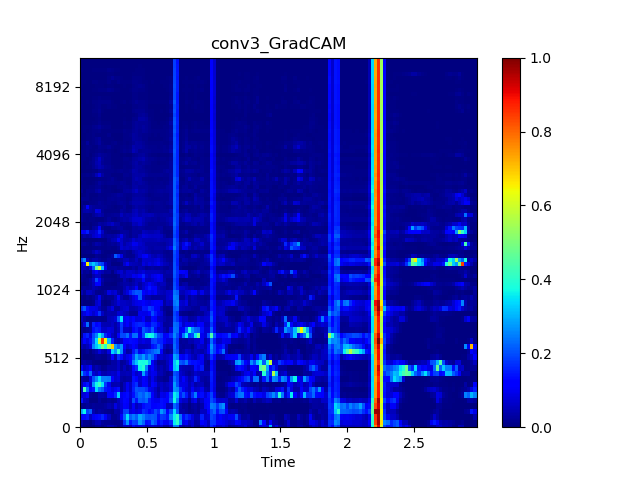
\includegraphics[scale=0.7]{./images/appendix/6_gradcam.png}
		\caption{Grad-CAMによる入力スペクトログラムのヒートマップ化}
		\label{fig:grad-cam-mel}
	\end{center}
\end{figure}


\figref{fig:grad-cam-mel}は\figref{fig:networkCNN}における3層目の畳み込み層の特徴マップの勾配を平均化した際のヒートマップ出力を表している.このとき,特徴マップの大きさが(1, 118)であるためヒートマップ出力が縦長になってしまっていることがわかる.このことから数値的にクラスの確率を上げるために入力データの重要な箇所を特定することはできるが,人間が解釈可能ではないヒートマップ出力となってしまっている.

\chapter{MNISTを用いた予備実験}
手書き数字データセットMNISTを用いたときの二次元ジャンルマップを作成する.この時のジャンルマップの変化と確率変化を動画にしたものを以下のURLに掲載する.\\
\url{https://github.com/hayashi-labratory/yamakawa_master_paper_sorcecode/tree/master/images}
